\startchapter{Simplified Molecule} \label{ch:3}

\section{Description}
The goal of Chapter \ref{ch:3} is to introduce the formulas used to describe our LP model. As well as exploring the properties of our LP model by using a simplified molecule. This simplified molecule contains limited vibration modes. By doing so, the nature of the LP model we use to study the spectral information can be carefully analyzed. Our goal is to figure out with the spectral information available, could LP model we use extract any valuable information. \\

The simplified molecule contains $4$ vibration modes. Theses vibrational peaks are at frequencies of $2850$, $2960$, $3050$ and $3200~\rm cm^{-1}$. The widths of the peaks are $5$, $10$, $5$ and $15~\rm cm^{-1}$, respectively. The amplitudes of the peak are $1$, $0.7$, $-0.2$ and $0.5~\rm cm^{-1}$, respectively. The comparing angles of the peaks are $15^{\circ}, 90^{\circ}, 0^{\circ}$ and $60^{\circ}$. \\

Because we want to limit the complexity that comes from the parameters needed to describe the realistic molecules. Only IR spectroscopy is considered for the simplified molecule. Equation \ref{eq:3.1} is used to generate the $z$-polarized IR spectrum. Moreover, both $\phi$ and $\psi$ Euler angles are integrated, only the difference on angle $\theta$ is considered. \\

\begin{eqnarray} \label{eq:3.1}
& f_{\theta}(\omega_{\rm IR}) = \displaystyle\sum^{4}_{q=1} A_q^2 cos^2(\theta - \theta_q)\frac{\Gamma^2}{(\omega_{\rm IR}- \omega_{\rm q})^2 + \Gamma^2} 
\end{eqnarray}
where $A_{q}$ is the amplitude, $\theta_{q}$ is the comparing angle, $\Gamma$ is the width, and $\omega_{\rm q}$ is the frequency. Ten candidates are produced with $10$ different $\theta$ values as follows: $0^{\circ}$, $10^{\circ}$, $20^{\circ}$, $30^{\circ}$, $40^{\circ}$, $50^{\circ}$, $60^{\circ}$, $70^{\circ}$, $80^{\circ}$, $90^{\circ}$. Their spectra are shown in Figure \ref{fig:3.1}. The 10 candidates have peaks at the same frequencies. The spectral signal for candidates is comparatively strong at each peak. \\

\begin{figure}[!ht] 
\centering
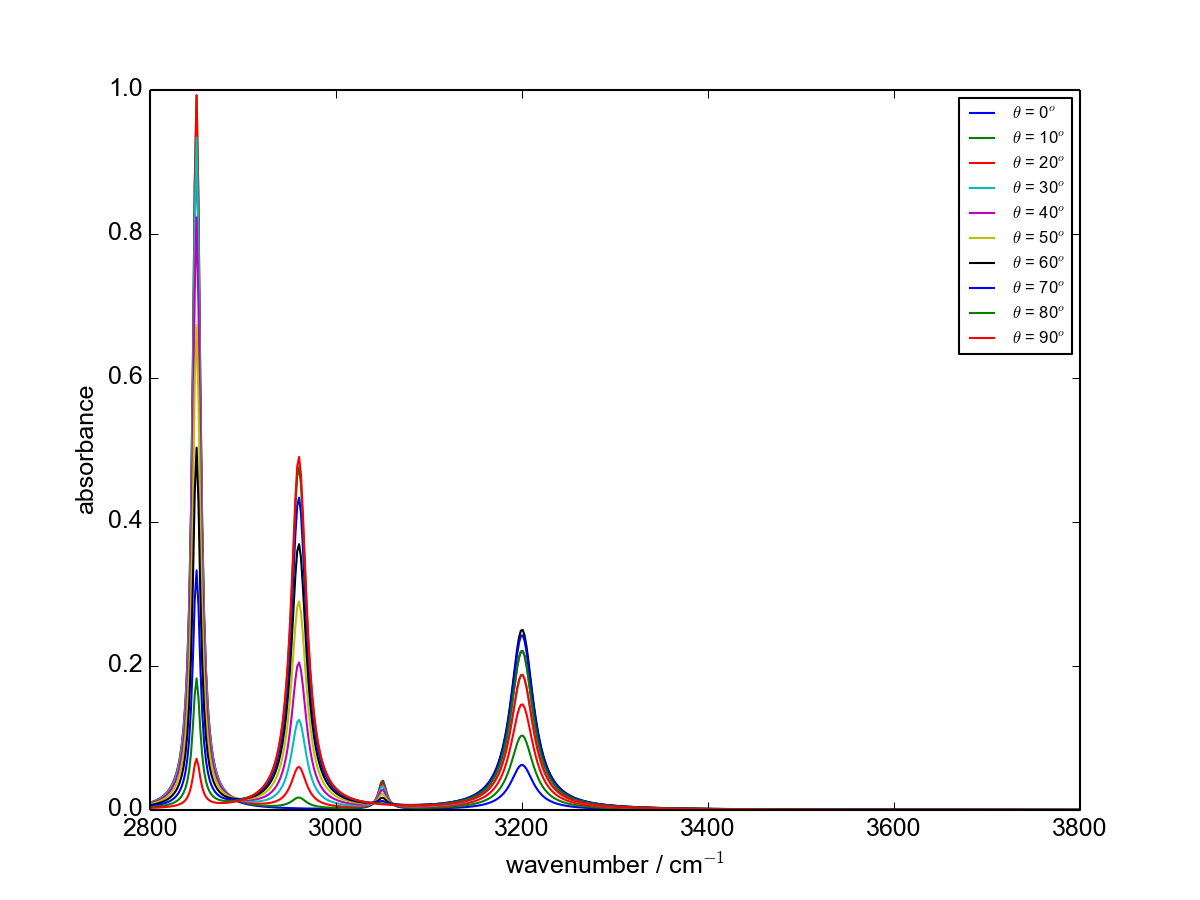
\includegraphics[scale=0.7]{Figures/Toy_Model_IR_Cosine_Projection.png} 
\caption{$z$-polarize IR spectra of simplified molecule candidates} \label{fig:3.1}
\end{figure}

%A target spectrum is composed by combining $15$ percent of candidate with $\theta$ of $20^{\circ}$ and $85$ percent of candidate of $\theta$ of $70^{\circ}$: $0.15*f_{20}(x) + 0.85*f_{70}(x)$ in the following experiment. \\

\section{Linear Programming Model for Spectral Study}

Equation \ref{eq:3.2} is used to construct our LP model. The optimal solution returned by the LP solver is then compared with the target composition to see if they match each other. This equation has also been used to study the composition of Ribonucleic acid (RNA) with ultraviolet (UV) spectra \cite{NYAS:NYAS900} and other UV spectroscopy studies  \cite{LPATUAS} back in the 60s. \\

\begin{eqnarray} \label{eq:3.2}
& \underset{p_{c}} {\text{minimize}} \displaystyle\sum^{N_{p}}_{n=1} \left| \rm Target- \displaystyle\sum^{N_{c}}_{c=1}p_{c}f_{\theta}(x) \right| 
\end{eqnarray}
where $p_{c}$ are the unknown percentages for each candidate, which are the decision variables. $n$ is the number of points $N_{p}$ selected along the wavenumber, both for candidates and target spectra. $\rm Target$ refers to the corresponding data points selected in target spectra. $N_{c}$ is the number of candidates. For each data point, the absolute residual between the target spectrum and the one composed by the decision variables is calculated. The objective function minimizes the sum of the absolute residuals over all the data points. \\

However, because of the absolute signs in the objective function, Equation \ref{eq:3.2} is not in an LP problem. Getting rid of the absolute signs is needed in order to use an LP approach. It is achieved by introducing one more variable $\rm X$ and two more constraints for each data point as shown in Equation \ref{eq:3.3}. The previous model in Equation \ref{eq:3.2} is then converted into the one in Equation \ref{eq:3.4}, and it can be solved by an LP solver. At last, one more constraint is introduced to restrict the sum of the percentages to be 1, as shown in Equation \ref{eq:3.4}. \\

\begin{eqnarray} \label{eq:3.3}
& X = \left| \rm Target-\displaystyle\sum^{N_{p}}_{c=1}p_{c}f_{\theta}(x) \right| \nonumber \\
&  X \geq \rm Target-\displaystyle\sum^{N_{c}}_{c=1}p_{c}f_{\theta}(x)   \nonumber \\
& X \geq -\rm Target+\displaystyle\sum^{N_{c}}_{c=1}p_{c}f_{\theta}(x)  
\end{eqnarray} 

\begin{eqnarray} \label{eq:3.4}
& minimize \displaystyle\sum^{N_{p}}_{n=1} X_p \nonumber \\
& \rm X_1 - \rm Target_1 + \displaystyle\sum^{N_{c}}_{c=1}p_{c}f_{\theta}(x_1) \geq 0 \nonumber \\
& \rm X_1 + \rm Target_1 - \displaystyle\sum^{N_{c}}_{c=1}p_{c}f_{\theta}(x_1) \geq 0 \nonumber \\
&\vdots  \nonumber \\
& \rm X_n - \rm Target_n + \displaystyle\sum^{N_{c}}_{c=1}p_{c}f_{\theta}(x_n) \geq 0 \nonumber \\
& \rm X_n + \rm Target_n - \displaystyle\sum^{N_{c}}_{c=1}p_{c}f_{\theta}(x_n) \geq 0 \nonumber \\
& \displaystyle\sum^{N_{c}}_{c=1}p_{c} = 1 
\end{eqnarray} 

Note that our LP model exactly describes our problem to be solved. Assuming that we can obtain sufficiently precise data, solving the LP will yield the target composition. Recall if the solution space is feasible and bounded, then there is a unique optimum solution. \\

\section{Linear Programming Model Implementation}

Next, we describe how to solve Equation \ref{eq:3.4} by implementing our LP model. Code is written to generate a file that contains all the candidates' spectral information needed for the test cases. For this step, the molecular properties files that generated by the electronic structure calculations are used. For a specific candidate, given the electronic structure calculations and a $\theta$ value, the candidate's spectral information is obtained. To further illustrate, a candidate class is written. This class defines candidate's $x$- and $z$-polarized IR spectra; $xx$-, $xy$-, $xz$-, and $zz$-polarized Raman spectra; $xxz$-, $xzx$-, $zzz$-polarized SFG spectra. Given a candidate's molecular properties and a $\theta$ value, a instance of this specific candidate is created. For the simplified molecule, it only contains IR spectral information. Therefore, one candidate only contains $x$- and $z$-polarized IR spectra. \\

In the second step, more code is written to generate a target composition of a list of needed candidates. Then the target composition is used to generate the target spectra. The probe range, which is the range of the wavenumber, is from 2800 to 3300 for the                    simplified molecule. The probe arrange is from $2000$ to $3000~\rm cm^{-1}$ wavenumber for realistic molecules. It is from $2800$ to $3300~\rm cm^{-1}$ wavenumber for realistic molecules. The target spectral information is generated in the same text file as candidate's spectral information. Depend on the test case setting, code can be used to generate text files that contain selected types of spectral information. \\

In the third step, the LP model is constructed by using the spectral information text file generated in the second step. This part of the code was written by Hung \cite{KuoKaiHung:Thesis:2015}. It reads all the candidates and target spectral information, and builds the LP model as shown in Equation \ref{eq:3.4}, then creates LP input file. \\

In the fourth step, we use LP solver ``GNU linear progarmming tool kit" (GLPK) to read the LP input file, then obtain the result. \\

\section{Test Cases}

In Case 1 and 2, $4$ candidates are selected, the detailed setting is shown in Table \ref{tab:3.1}. In Case 1, there are $4$ candidates with $\theta$ of $0^{\circ}, 10^{\circ}, 20^{\circ}$, and $30^{\circ}$. In Case 2, the four candidates are with $\theta$ values of $0^{\circ}, 5^{\circ}, 10^{\circ}$, and $15^{\circ}$. Instead of having a $10$ degree variance in $\theta$, $5$ degree difference is applied on $\theta$ in Case 2. This means that when the candidates become more similar to each other than the ones in Case 1 as their spectra are more similar. In both cases, 100 data points are selected evenly along the wavenumber from the spectra of $z$-polarized IR. The target composition of the candidates are the same for both cases. In Case 1, the return composition is the same as the target one, however, the return composition for Case 2 does not match the target one. \\

\begin{table} 
\begin{center}
{\def\arraystretch{1.5}
\begin{tabular}{| l | l | l | }
\hline
Test Case index & 1 & 2  \\
\hline
Number of Candidates & 4 & 4  \\
\hline
Candidates & [0, 10, 20, 30] & [0, 5, 10, 15] \\
\hline
Target Composition & [0.1, 0.5, 0.4, 0] & [0.1, 0.5, 0.4, 0]     \\
\hline
Number of Data Points & 100, $z$ &  100, $z$     \\
\hline
%Return Composition & [0.1, 0.5, 0.4, 0] & [0, 0.796962, 0.103038, 0.1] \\
Return Composition & [0.1, 0.5, 0.4, 0] & [0, 0.80, 0.10, 0.1] \\
\hline
\end{tabular} 
}
\end{center}
\caption{Test case 1 and 2 setting using simplified molecule}
\label{tab:3.1}
\end{table}	

In order to figure out why the return composition in Case 2 is different from the target one, the spectra generated by the return composition is plotted together with the target spectra as shown in Figure \ref{fig:3.2}. Note that the result spectra is almost identical to the target one. The residual between them is almost $0$. In order to see whether this observation is a general case, Case 3 is set up in Table \ref{tab:3.2}. Case 3 contains more candidates than Cases 1 and 2. $10$ candidates are included with $\theta$ values ranging from $0^{\circ}$ to $90^{\circ}$.  \\

\begin{figure}[!ht] 
%\centering
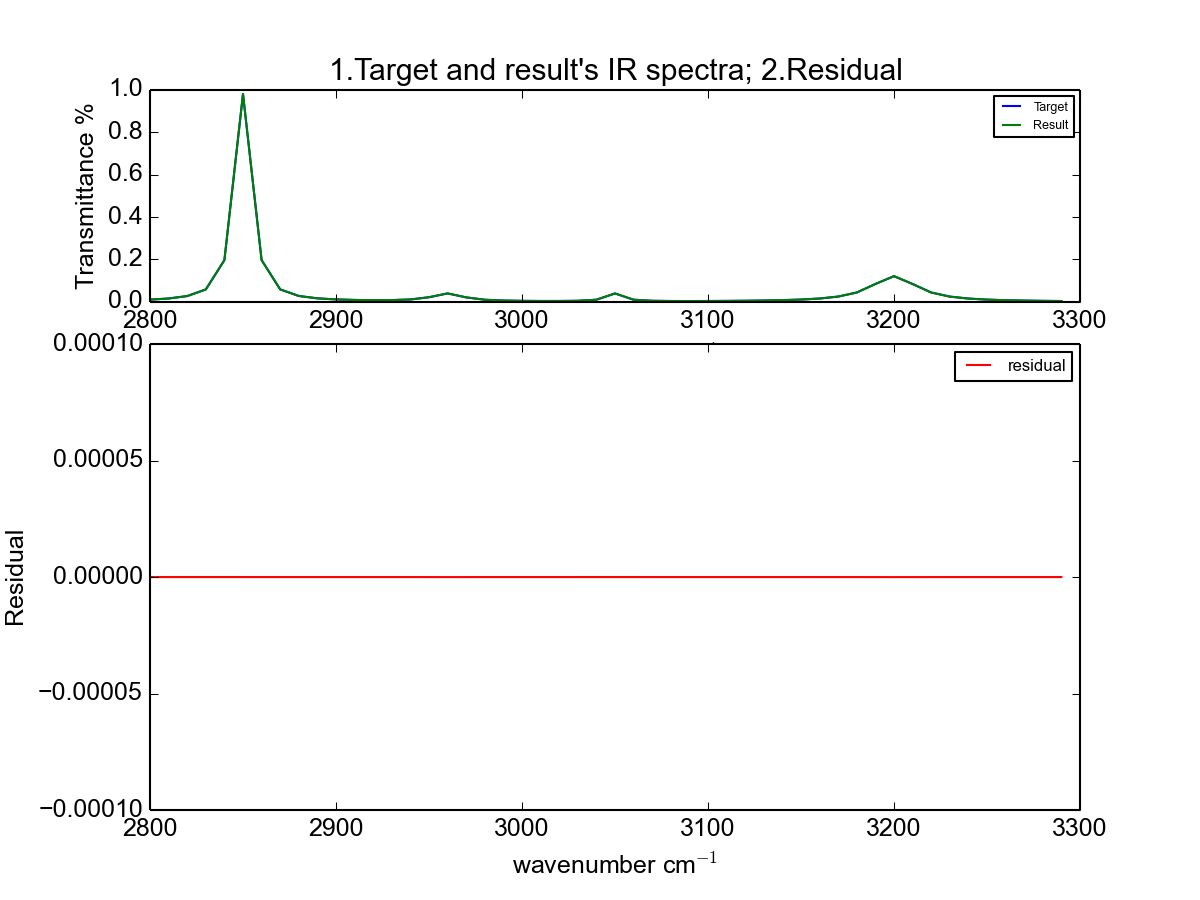
\includegraphics[scale=0.7]{Figures/toy_model_result_plotting_ir_cos_4candi_1.png}
\caption{a. simplified molecule Case 2 resulting $z$-polarized IR spectrum plotted with the target spectrum; b. the residual plot between the spectra.}
\label{fig:3.2}
\end{figure}

\begin{table} 
\begin{center}
\begin{tabular}{| l | p{7cm} | }
\hline
Test Case index & 3  \\
\hline
Number of Candidates & 10   \\
\hline
Candidates & [0, 10, 20, 30, 40, 50, 60, 70, 80, 90]  \\
\hline
Target Composition & [0.1, 0, 0.5, 0, 0.4, 0, 0, 0, 0, 0] \\
\hline
Number of Data Points & 100, $z$ \\
\hline
%Return Composition & [0, 0, 0.730541, 0, 0.212061,0, 0, 0.0573978, 0, 0] \\
Return Composition & [0, 0, 0.73, 0, 0.21,0, 0, 0.057, 0, 0] \\
\hline
\end{tabular}
\end{center}
\caption{Test case 3 setting of simplified molecule}
\label{tab:3.2}
\end{table}	

\begin{figure}[!ht] 
\centering
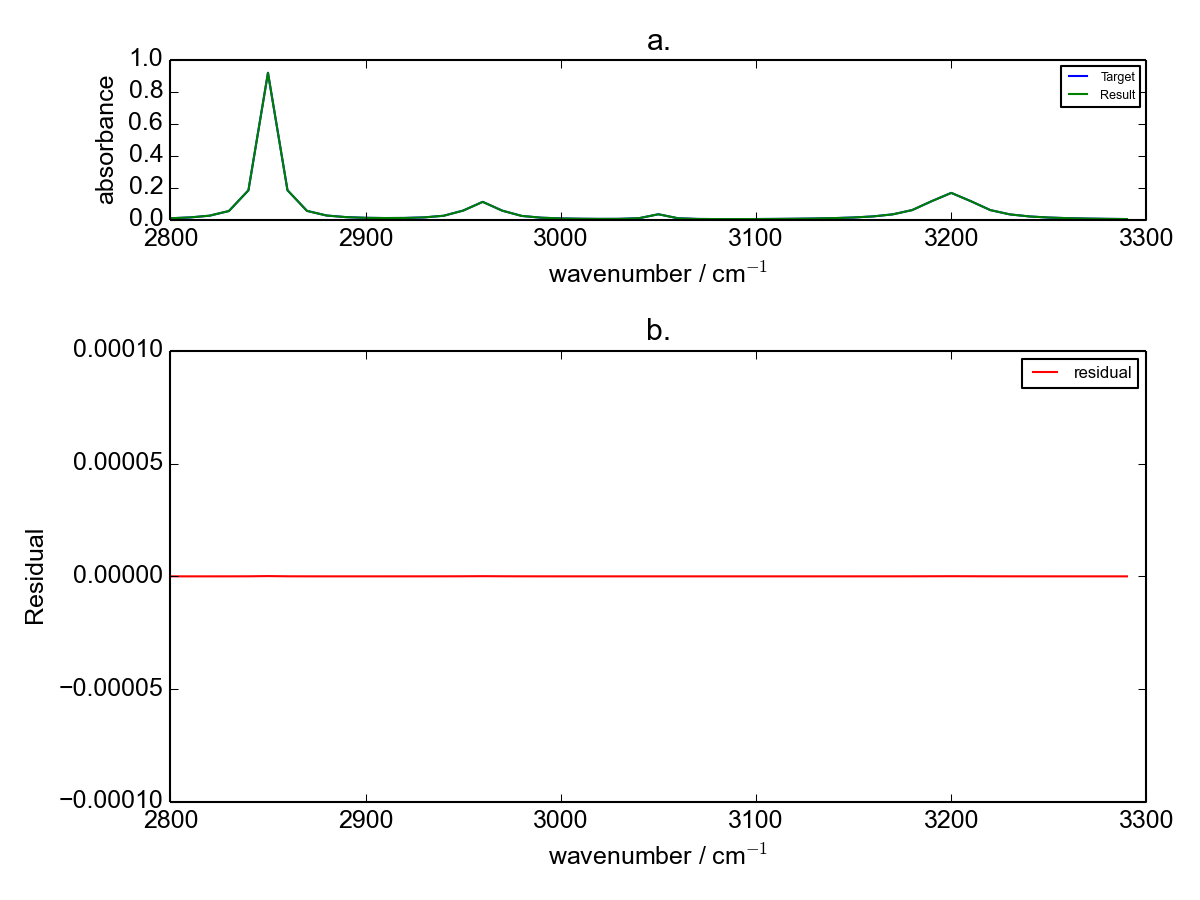
\includegraphics[scale=0.7]{Figures/toy_model_result_plotting_ir_cos_10candi_1.png} 
\caption{a. simplified molecule Case 3 resulting $cosine$-polarized IR spectrum plotted with target spectrum; b. the residual plot between the two spectra}
\label{fig:3.3}
\end{figure}

Table \ref{tab:3.2} indicates the return composition of Case 3 is different from the target one. Figure \ref{fig:3.3} shows that the spectrum produced by the return composition is almost identical to the one generated by the target composition in Case 3. The residual is negligible as well. This observation is the same as Case 2. \\

Among Case 1, 2 and 3, only the return composition of Case 1 matches its target one. However, in Case 2, the difference in $\theta$ value among the candidates is smaller than Case 1. In Case 3, the number of the candidates is larger than Case 1. Both effects increase the complexity of the cases. In both Case 2 and 3, the spectrum constructed by the return composition matches to the one built by the target composition. \\

The above observation demonstrates that there are multiple compositions can achieve in constructing the spectrum that are close to the target one. The numerical limitation helps the LP solver to converge to a unique optimum solution. The reason for Case 1 to return a composition that matches to the target one, is that the spectral information applied to the LP model is competent. The constraints constructed in the LP model of Case 1 eventually converge to the target composition. \\ 

In order to add necessary information to construct the constraints in our LP model, IR's second polarization is introduced to the simplified molecule: the $x$ polarization. Figure \ref{fig:3.4} describes how the $x$-polarized spectra presented for $10$ candidates. Test Case 4 and 5 include both polarizations' spectral information in the LP model. In Table \ref{tab:3.3}, Case 4's setting is based on Case 2, with $x$-polarized IR spectral information added. $100$ data points are selected from this additional spectrum, then converted to additional decision variables and constraints in the LP model. Case 5 is based on Case 3, with $x$-polarized IR spectral information added. In both Case 4 and 5, the return composition matches to the target one. This further proves that as long as we have sufficing information for the LP model, the LP solver returns a composition matches to the target one. \\ 

\begin{figure}[!ht]
\centering
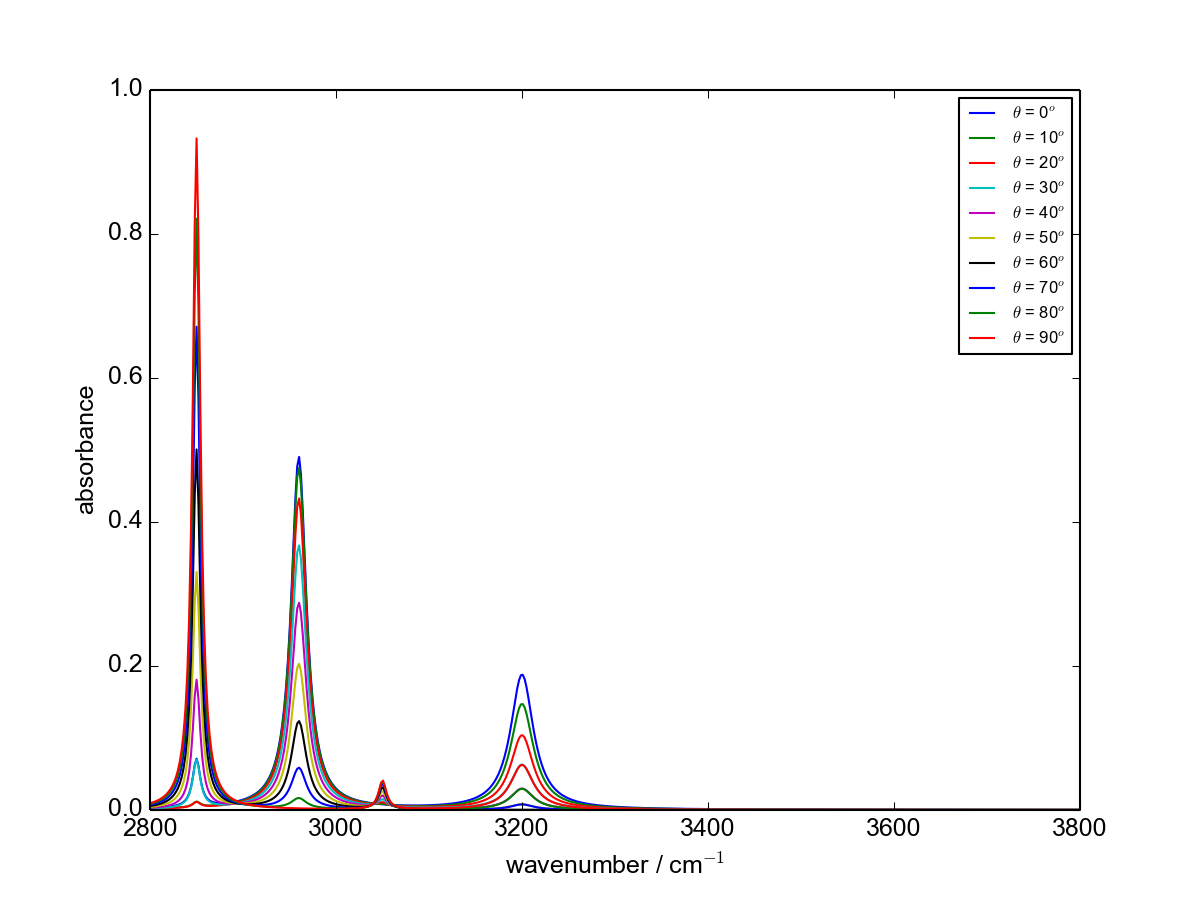
\includegraphics[scale=0.7]{Figures/Toy_Model_IR_Sine_Projection.png} 
\caption{$x$-polaried IR spectra of simplified molecule candidates with $\theta$ value expanded from $0^{\circ}$ to $90^{\circ}$}  \label{fig:3.4}
\end{figure}

\begin{table} \small 
\begin{center}
{\def\arraystretch{1.5}
\begin{tabular}{| l | p{3cm} | p{6cm} |}
\hline
Test Case index & 4 & 5\\
\hline
Number of Candidates & 4 & 10 \\
\hline
Candidates & [0, 5, 10, 15] & [0, 10, 20, 30, 40, 50, 60, 70, 80, 90] \\
\hline
Target Composition & [0.1, 0.5, 0.4, 0] & [0.1, 0, 0.5, 0, 0.4, 0, 0, 0, 0, 0]\\
\hline
Number of Data Points & 100, $z$ \newline 100, $x$ & 100, $z$ \newline 100, $x$\\
\hline
Return Composition & [0.1, 0.5, 0.4, 0] & [0.1, 0, 0.5, 0, 0.4, 0, 0, 0, 0, 0] \\
\hline
\end{tabular}
} 
\caption{Test case 4 and 5 setting of simplified molecule}\label{tab:3.3}
\end{center}
\end{table}		

\section{Constraint Study Based on Test Case 4}

From Case 1 to 5 of simplified molecule, we know having sufficient information in our LP model is the key to obtain the target composition. Having sufficient information means having enough constraints to help to converge to the desired target composition. The information is coming from the data points selected along the spectra. This leads us to do a more detailed study on the constraints in order to see how many data points are enough to get the target composition.\\ 

Based on Case 4, cases about applying different data information to the LP model are conducted in Table \ref{tab:3.4}. The number of data points indicates how many data points are selected. Points Selection shows how data points are selected. For example, [2800, 3300, 50] means along wavenumber from 2500 to 3300, every 50 wavenumber a data point is selected along a spectrum. $z$ and $x$ indicate the corresponding polarization of IR spectrum. \\

\begin{table} \small
\begin{center}
{\def\arraystretch{1.5}
\begin{tabular}{| p{3cm} | p{3cm} | p{4cm} | l |} \hline
	Test Case \# & \# Data Points & Points Selection & Return Composition \\ \hline
	6 & 10 & [2800, 3300, 50], $z$ & [0, 0.8, 0.10, 0.1] \\ \hline
	7 & 20 & [2800, 3300, 25], $z$ & [0, 0.8, 0.10, 0.1 \\ \hline
	8 & 25 & [2800, 3300, 20], $z$ & [0, 0.8, 0.10, 0.1] \\ \hline
	9 & 32 & [2800, 3300, 15], $z$ & [0, 0.8, 0.10, 0.1] \\ \hline
	10 & 50 & [2800, 3300, 10], $z$ & [0, 0.8, 0.10, 0.1] \\ \hline
	11 & 100 & [2800, 3300, 5], $z$ & [0, 0.8, 0.10, 0.1] \\ \hline
	12 & $100 + 1$ & [2800, 3300, 5], $z$ \newline [2800, 3300, 500], $x$ & [0, 0.8, 0.10, 0.1] \\ \hline
	13 & $100 + 5$ & [2800, 3300, 20], $z$ \newline [2800, 3300, 100], $x$ & [0, 0.8, 0.10, 0.1] \\ \hline
	14 & $100 + 10$ & [2800, 3300, 20], $z$ \newline  [2800, 3300, 50], $x$ & [0, 0.8, 0.10, 0.1] \\ \hline
	15 & $100 + 50$ & [2800, 3300, 20], $z$ \newline  [2800, 3300, 10], $x$ & [0.1, 0.5, 0.4, 0] \\ \hline
	16 & $100 + 100$ & [2800, 3300, 20], $z$ \newline  [2800, 3300, 5], $x$ & [0.1, 0.5, 0.4, 0] \\ 
	\hline
\end{tabular} 
}
\end{center}
\caption{Constraint study based on Case 4 of simplified molecule. For more precise result data, refer Table \ref{tab:7.3}.} \label{tab:3.4}
\end{table}

As Table \ref{tab:3.4} indicates, the return compositions of Case 6 to 14 are the same. To the contrary, from Case 15, the return composition matches the target one. In Figure \ref{fig:3.5} displays the spectra conducted by $[0, 0.796962, 0.103038, 0.1]$ and $[0.1, 0.5, 0.4, 0]$, both $x$- and $z$-polarized IR spectra generated by these two compositions are identical.

\begin{figure}[!ht] 
\centering
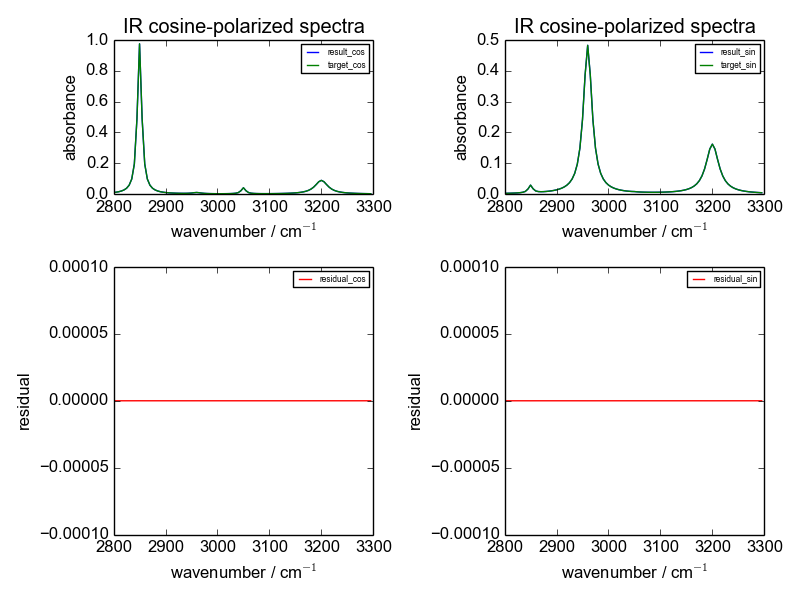
\includegraphics[scale=0.7]{Figures/toy_model_result_plotting_ir_sin_4candi_constraint_study_experiment4.png} 
\caption{IR spectra plotted by the return compositions from the constraint study based on Case 4 of simplified molecule}\label{fig:3.5}
\end{figure}


\section{Constraint Study Based on Test Case 5}

Based on Case 5, similar constraint study is conducted as displayed in Table \ref{tab:3.5}, and the same observation is obtained as the test cases in Table \ref{tab:3.4}. When the result composition $[0, 0, 0.730541, 0, 0.212061,0, 0, 0.0573978, 0, 0]$ and target one are used to plot the spectra, the produced spectra are almost identical as shown in Figure \ref{fig:3.6}.
%$[0, 0, 0.730541, 0, 0.212061,0, 0, 0.0573978, 0, 0]$
\begin{table} \small
\begin{center} 
{\def\arraystretch{1.5}
\begin{tabular}{| p{1cm} | p{2cm} | p{4cm}  | l |}
\hline
Test Case \# & \# of Data Points & Point Selection & Return Composition \\ \hline
17 & 10 & [2800, 3300, 50], $z$ & [0.16, 0, 0, 0.83, 0, 0, 0, 0, 0, 0.017] \\ \hline
18 & 25 & [2800, 3300, 20], $z$ & [0, 0, 0.73, 0, 0.21, 0, 0, 0.057, 0, 0, 0] \\ \hline
19 & 50 & [2800, 3300, 10], $z$ & [0, 0, 0.73, 0, 0.21, 0, 0, 0.057, 0, 0, 0] \\ \hline
20 & 100 & [2800, 3300, 5], $z$ & [0, 0, 0.73, 0, 0.21, 0, 0, 0.057, 0, 0, 0] \\ \hline
21 & 500 & [2800, 3300, 1], $z$ & [0, 0, 0.73, 0, 0.21, 0, 0, 0.057, 0, 0, 0] \\ \hline	
22 & $100 + 1$ & [2800, 3300, 5], $z$ \newline [2800, 3300, 500], $x$  & [0, 0, 0.73, 0, 0.21, 0, 0, 0.057, 0, 0, 0] \\ \hline
23 & $100 + 10$ & [2800, 3300, 5], $z$ \newline [2800, 3300, 50], $x$  & [0.36, 0, 0.31, 0.33, 0, 0, 0, 0, 0] \\ \hline
24 & $100 + 20$ & [2800, 3300, 5], $z$ \newline [2800, 3300, 25], $x$  & [0.17, 0, 0, 0.79, 0, 0, 0.035, 0, 0, 0] \\ \hline
25 & $100 + 25$ & [2800, 3300, 20], $z$ \newline [2800, 3300, 20], $x$  & [0.17, 0, 0, 0.79, 0, 0, 0.035, 0, 0, 0] \\ \hline
26 & $100 + 50$ & [2800, 3300, 5], $z$ \newline [2800, 3300, 10], $x$  & [0, 0, 0.75, 0, 0.15, 0, 0.1, 0, 0, 0] \\ \hline
27 & $100 + 84$ & [2800, 3300, 5], $z$ \newline [2800, 3300, 6], $x$  & [0.17, 0, 0, 0.79, 0, 0, 0.035, 0, 0, 0] \\ \hline
28 & $100 + 100$ & [2800, 3300, 5], $z$ \newline [2800, 3300, 5], $x$  & [0.1, 0, 0.5, 0, 0.4, 0, 0, 0, 0, 0] \\ 
\hline
\end{tabular} \\
}
\caption{Constraint study based on Case 5 of simplified molecule. For more precise result data, refer Table \ref{tab:7.4}.}\label{tab:3.5}
\end{center}
\end{table}

\begin{figure}[!ht] 
\centering
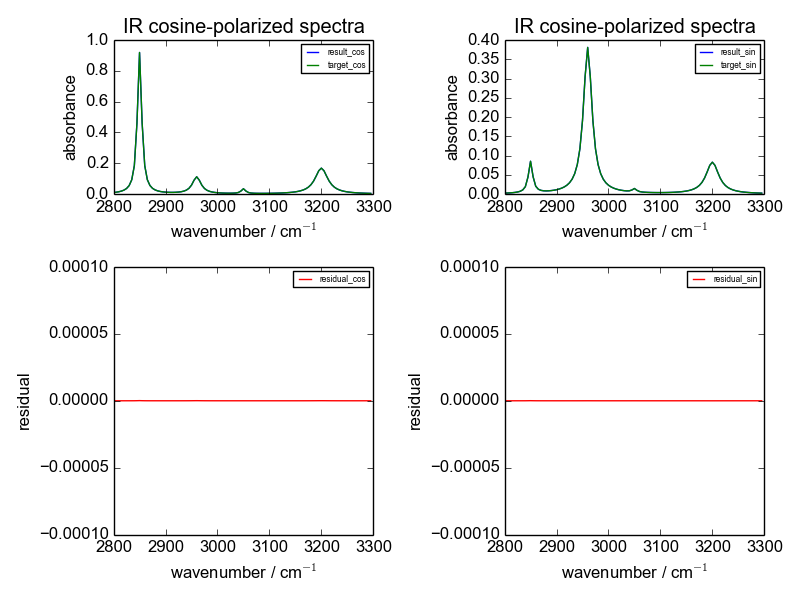
\includegraphics[scale=0.7]{Figures/toy_model_result_plotting_ir_sin_10candi_constraint_study_experiment5.png} 
\caption{IR spectra plotted by the return compositions from the constraint study based on Case 5 of simplified molecule}\label{fig:3.6}
\end{figure}

\section{Discussion and Conclusion}

Recall that our LP model, for the right data set is expected to return the target composition. We can conclude that, if the target composition is not returned correctly, then the data we collect is not sufficient to describe the test cases to the LP model. \\

However, when the target composition is not returned correctly, the return composition does build spectra that are almost identical to the target ones. This means that there are more than one composition can build the spectra that are almost identical to the target ones. Because of the numerical limitation, an unique optimum solution is always obtained. \\

The above conclusion leaves us a new question: how do we know there is sufficient spectral information in order to obtain the target composition of candidates at interfaces? To answer this question, further test cases are conducted by applying the spectral information of realistic molecules to the LP model. The goal is to investigate with all the spectral information we can obtain for realistic molecules, can the LP model return the target composition of candidates at interfaces. If this goal can be achieved, can this approach be applied systematically to different circumstances?

%Above analysis simulates the following question: how can we know there is enough information to achieve the target composition? In the next step, we will experiment with real molecules. The goal is to investigate with all the spectral information that we can obtain for real molecules, can our LP model return the target composition for the target spectrum? If yes, can we apply the LP model systematically? Furthermore, to maximally explore the capacity of our LP model, and study its limitation. Finally, come up with some general instructions for applying our LP model. These are the main focus for the following chapters.\\

		

		 



